\section{Diagramma delle classi}
In questo capitolo vengono presentate e descritte le classi, che sono richieste per lo sviluppo dell'applicazione JGuesser. Tutte le classi sono costituite da un insieme di attributi e metodi. Gli attributi rappresentano i dati su cui la classe dovrà operare. I metodi sono invece le funzionalità che la classe può offrire. Entrambi possono essere:
\begin{itemize}
    \item pubblici (+): l'attributo/metodo può essere accessibile dall'esterno della classe in cui è stato definito.
    \item privati (-): l'attributo/metodo può essere accessibile solo all'interno della classe in cui è stato definito.
    \item protetti (\#): l'attributo/metodo può essere accessibile solo all'interno della classe in cui è stato definito e nelle classi derivate.
\end{itemize}
\noindent
Nel nostro caso però non sono stati utilizzati, perchè discutendo ci siamo resi conto, che sono specifiche di programmazione e non di progettazione, esattamente come i getters/setters. \\
Le classi inoltre possono essere messe in relazione tra di loro ed è possibile associarvi una molteplicità. Una relazione tra due classi rappresenta il fatto che le due classi interagiscono fra di loro e si scambiano dei dati. \\
Per individuare le classi quello che è stato fatto è partire dal diagramma delle componenti e di contesto. Questo perchè di solito una componente del diagramma delle componente viene mappata in una o più classi e un attore del diagramma di contesto può essere mappato in una classe (es: user). Siccome le classi coinvolte nel diagramma del progetto JGuesser sono tante, si è optato per spezzettare la descrizione in una o gruppi di classi, un po' come è stato fatto per gli use-case diagram.

\newpage
\subsection{Utente}
Analizzando il diagramma del contesto del progetto JGuesser è possibile individuare gli attori: 
\begin{itemize}
    \item Guest: non bisogna salvare alcun dato per lui;
    \item Utente registrato: bisogna salvare una serie di dati;
    \item Utente premium: non bisogna salvare dati aggiuntivi all'utente registrato, in quanto l'utente premium avrà accesso semplicemente a funzionalità aggiuntive, che non produrranno però dati aggiunitvi da memorizzare.
\end{itemize} 
Per questo motivo si è optato in fase di progettazione del diagramma delle classi, di fare una classe singola e di non utilizzare l'erditarietà (generalizzazione). Oltre ai dati da memorizzare per l'utente questa classe contiene anche una serie di metodi, che servono ad effettuare dei controlli su come i dati sono formattati. Questi metodi sono utili per effettuare dei controlli preventivi nel front-end ed evitare di interrogare il back-end, per cose che si potrebbero fare benissimo lato client.

\begin{figure}[!h]
\centering
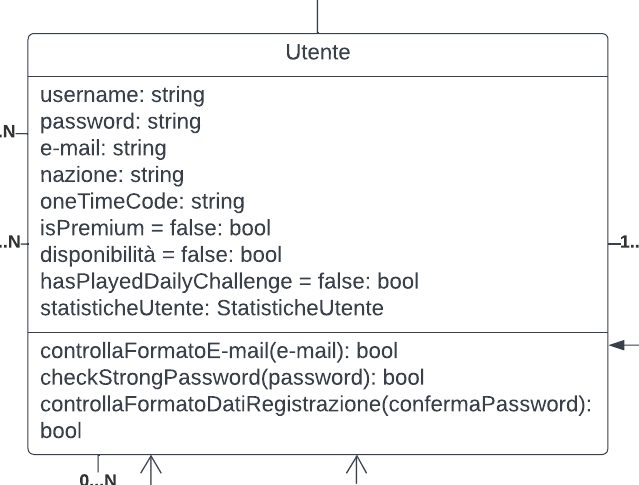
\includegraphics[scale=0.35]{images/classe_utente.png}
\caption{Classe per i dati dell'utente}
\label{fig:classe_utente}
\end{figure}
\noindent

\newpage
\subsection{Sistema di invio e-mail}
Analizzando il diagramma delle componenti del progetto JGuesser è possibile individuare la componente InterfacciaNodemailer, che si interfaccerà con il corrispettivo sistema esterno. Questa componente è stata trasformata nella seguente classe:

\begin{figure}[!h]
\centering
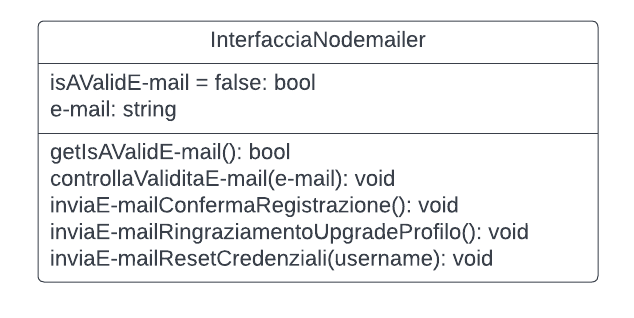
\includegraphics[scale=0.35]{images/classe_interfaccia_nodemailer.png}
\caption{Classe InterfacciaNodemailer}
\label{fig:classe_interfaccia_nodemailer}
\end{figure}
\noindent
Questa classe sarà quella che verrà utilizzata per verificare la validità di un e-mail, attraverso il metodo controllaValiditàE-mail(e-mail). Tale metodo andrà quindi a settare le variabili e-mail e isAValidE-mail, a cui poi sarà possibile accedere. Oltre a ciò questa classe ha il compito di inviare tutte le e-mail che l'applicazione necessita di spedire.

\subsection{reCAPTCHA}
Analizzando il diagramma delle componenti del progetto JGuesser è possibile individuare la componente Validatore reCAPTCHA, che si interfaccerà con il corrispettivo sistema esterno. Questa componente è stata trasformata nella seguente classe:

\begin{figure}[!h]
\centering
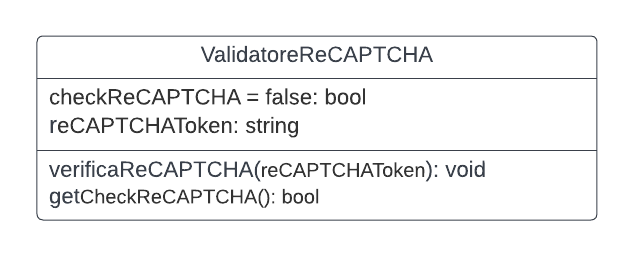
\includegraphics[scale=0.35]{images/classe_validatore_recaptcha.png}
\caption{Classe ValidatoreReCAPTCHA}
\label{fig:classe_validatore_recaptcha}
\end{figure}
\noindent
Tale classe si occuperà di ricevere i reCAPTCHAToken e di verificare attraverso il metodo verificaReCAPTCHA() la corretta esecuzione del test reCAPTCHA. Questo metodo andrà quindi a settare le variabili checkReCAPTCHA e reCAPTCHAToken, a cui sarà possibile accedere.

\newpage
\subsection{Registrazione e autenticazione}
Osservando il diagramma delle componenti del progetto JGuesser è possibile individuare tre componenti: 
\begin{itemize}
    \item Gestore registrazione: era quella componente che si occupava di gestire la registrazione di un determinato utente all'interno del sistema. Si è deciso di creare per questa componente una classe chiamata Registrazione, che permetterà all'utente di registrarsi; 
    \item Autenticazione: era quella che si occupava di gestire il login con le sole credenziali e si è deciso di creare una classe per tale componente;
    \item Autenticazione con Google: era quella che si interfacciava con il sistema esterno "Google Identity Service". Data la sua semplicità si è deciso in fase di progettazione del diagramma delle classi di far collassare tutte le funzionalità di quella classe, nella classe autenticazione, che gestisce anche il login con credenziali.
\end{itemize}
\noindent
 
\begin{figure}[!h]
\centering
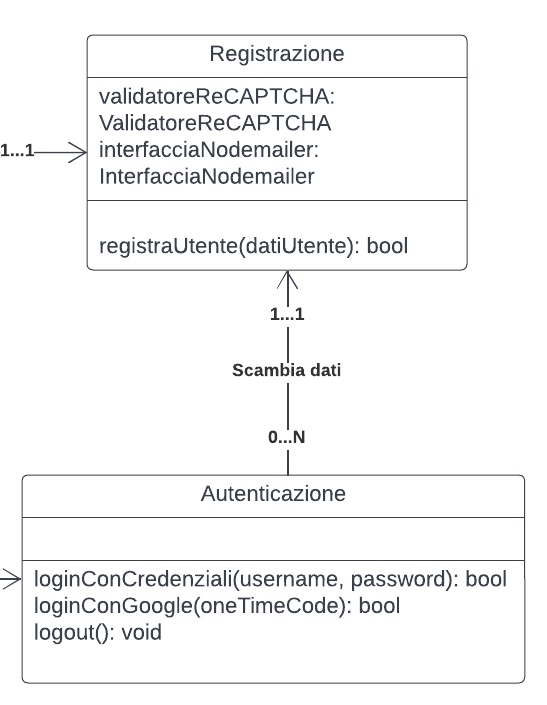
\includegraphics[scale=0.35]{images/classe_registrazione_autenticazione.png}
\caption{Classi per la registrazione e autenticazione}
\label{fig:classe_registrazione_autenticazione}
\end{figure}
\noindent
È stata inoltre identificata un associazione tra le due classi. Questo perchè nel caso in cui si effettui l'autenticazione utilizzando un account google, il sistema ha la necessità di registrare l'utente all'interno del database dell'applicazione, nel caso in cui non fosse gia stato fatto precedentemente. Per questo motivo la classe Autenticazione scambierà una serie d'informazioni (e-mail, token ecc...) con la classe Registrazione per registrare l'utente.

\newpage
\subsection{Modifica e reset credenziali}
Analizzando il diagramma delle componenti del progetto JGuesser è possibile individuare la componente Gestore credenziali, che si occupava di gestire la modifica e il reset delle credenziali dell'utente. In fase di progettazione del diagramma delle classi si è scelto di spezzare questa componente in due classi distinte:
\begin{itemize}
    \item ResetCredenziali: si occupa di gestire il solo reset delle credenziali dell'utente, nel caso in cui questo si fosse dimenticato l'username o la password. In questa classe sono presenti:
    \begin{itemize}
        \item un istanza della classe InterfacciaNodemailer: serve ad inviare l'e-mail di reset delle credenziali.
        \item un istanza della classe ValidatoreReCAPTCHA: serve a verificare che l'utente abbia cliccato il reCAPTCHA.
        \item il metodo resettaCredenziali: resetterà le credenziali dell'utente e invierà l'e-mail all'utente con le nuove credenziali (utilizzando interfacciaNodemailer).
    \end{itemize}
    \item ModificatoreCredenziali: si occupa di gestire la sola modifica dell'e-mail e la password dell'utente nel caso in cui questo sia capace di effettuare il login. In questa classe sono presenti:
    \begin{itemize}
        \item un istanza della classe Utente: verrà popolata con i dati dell'utente che verranno mostrati a video, nella propria area personale.
        \item una serie di attributi che servono a modificare l'e-mail o la password.
        \item un istanza della classe InterfacciaNodemailer: serve a controllare la validità di un e-mail.
        \item il metodo richiestaDatiUtente: serve a popolare l'istanza datiUtenteCorrente. Questo viene fatto effettuando un interrogazione al DB.
        \item il metodo effettuaModificaE-mail: serve a modificare l'e-mail dell'utente. Restituisce 'false' nel caso in cui l'e-mail inserita non è valida.
        \item il metodo effettuaModificaPassword: serve a effettuare la modifica della password. Restituisce 'false' nel caso in cui la procedura per modifcare la password non vada a buon fine.
    \end{itemize}
\end{itemize}

\begin{figure}[!h]
\centering
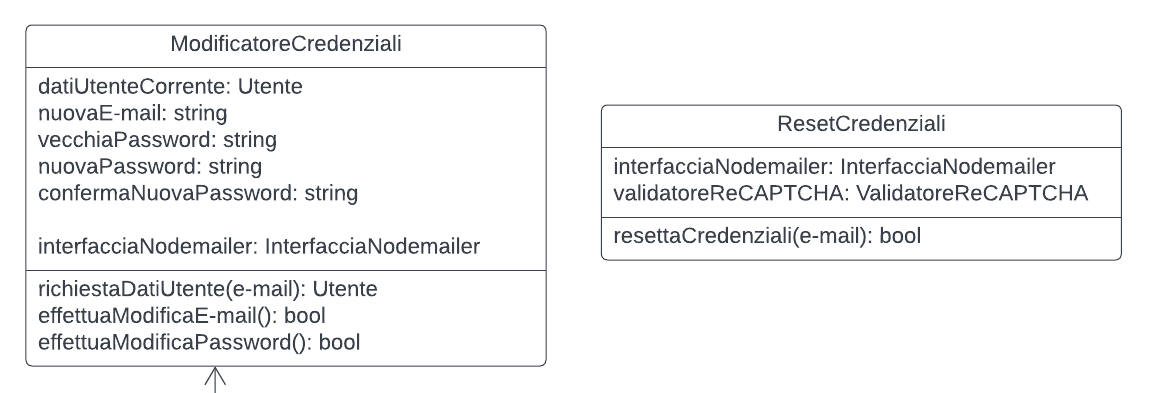
\includegraphics[scale=0.35]{images/classe_modifica_reset_credenziali.png}
\caption{Classi per gestire le credenziali}
\label{fig:classi_gestione_credenziali}
\end{figure}
\noindent

\subsection{Sistema di upgrade profilo}
Osservando il diagramma delle componenti del progetto JGuesser è possibile individuare le componenti:
\begin{itemize}
    \item Gestore pagamenti: si occupava di gestire i pagamenti interagendo con il sistema esterno Paypal; 
    \item Gestore upgrade profilo: si occupava di gestire la sola modifica dei privilegi di un utente (un update al database) e l'invio di un e-mail. Data la semplicità di questa componente, in fase di progettazione si è deciso di far collassare entrambe le componenti in un unica classe chiamata GestoreUpgradePremium.
\end{itemize}

\begin{figure}[!h]
\centering
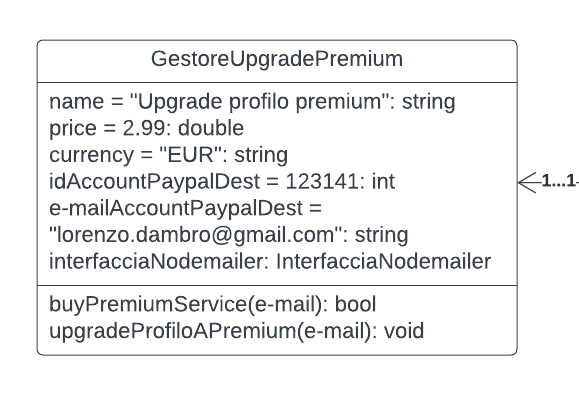
\includegraphics[scale=0.35]{images/classe_upgrade_profilo.png}
\caption{Classe per upgradare il profilo}
\label{fig:classe_upgrade_profilo}
\end{figure}
\noindent
Questa classe contiene come attributi tutti i dati necessari per effettuare la transazione e un istanza della classe InterfacciaNodemailer, che sarà utilizzata dal metodo upgradeProfiloAPremium per inviare un e-mail di ringranziamento per aver upgradato il proprio profilo. \\
Oltre a ciò sono presenti i metodi:
\begin{itemize}
    \item buyPremiumService: effettua il pagamento interagendo con il relativo sistema esterno.
    \item upgradeProfiloAPremium: aggiorna i permessi del profilo a premium ed invia l'e-mail di ringraziamento.
\end{itemize}

\subsection{Classifica e statistiche utente}
Analizzando il diagramma delle componenti del progetto JGuesser è possibile individuare la componente Gestore dati utente. Questa componente si occupava di gestire i dati da mostrare in classifica e le statistiche del singolo utente. Date queste due differenze in fase di proggettazione si optato per spezzare questa componente in due classi:
\begin{itemize}
    \item StatisticheUtente: si occupa di contenere tutti i dati relativi alle sole statistiche di un utente. Le statistiche di un singolo utente verranno richieste al database utilizzando il metodo richiediStatisticheUtente.
    \item Classifica: si occupa di contenere tutte le statistiche di tutti gli utenti che verranno visualizzati nella classifica. I dati degli utenti che verranno visualizzati in classifica possono essere richiesti tramite il metodo richiediDatiClassifica. I dati del singolo utente che si vuole filtrare nella classifica, verranno richiesti con il metodo richiediStatisticheUtenteSpecifico.
\end{itemize}

\begin{figure}[!h]
\centering
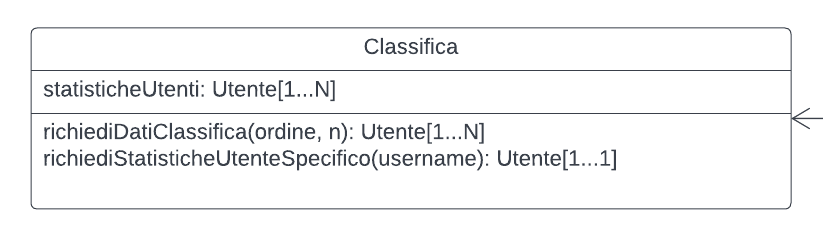
\includegraphics[scale=0.35]{images/classe_classifica.png}
\caption{Classe per la classifica}
\label{fig:classe_classifica}
\end{figure}
\noindent

%DA QUI MARCO IL SARDO
\subsection{QuizMaker, Quiz e Simbolo alfabeto}
Analizzando il diagramma delle componenti si può evincere la componente QuizMaker. Questa componente si interfaccia con il tipo di dato quiz, che a sua volta richiede i simboli dei vari alfabeti, per questo oltre alla classe QuizMaker sono state anche aggiunte le risorse Quiz e SimboloAlfabeto. 

\begin{figure}[!h]
\centering
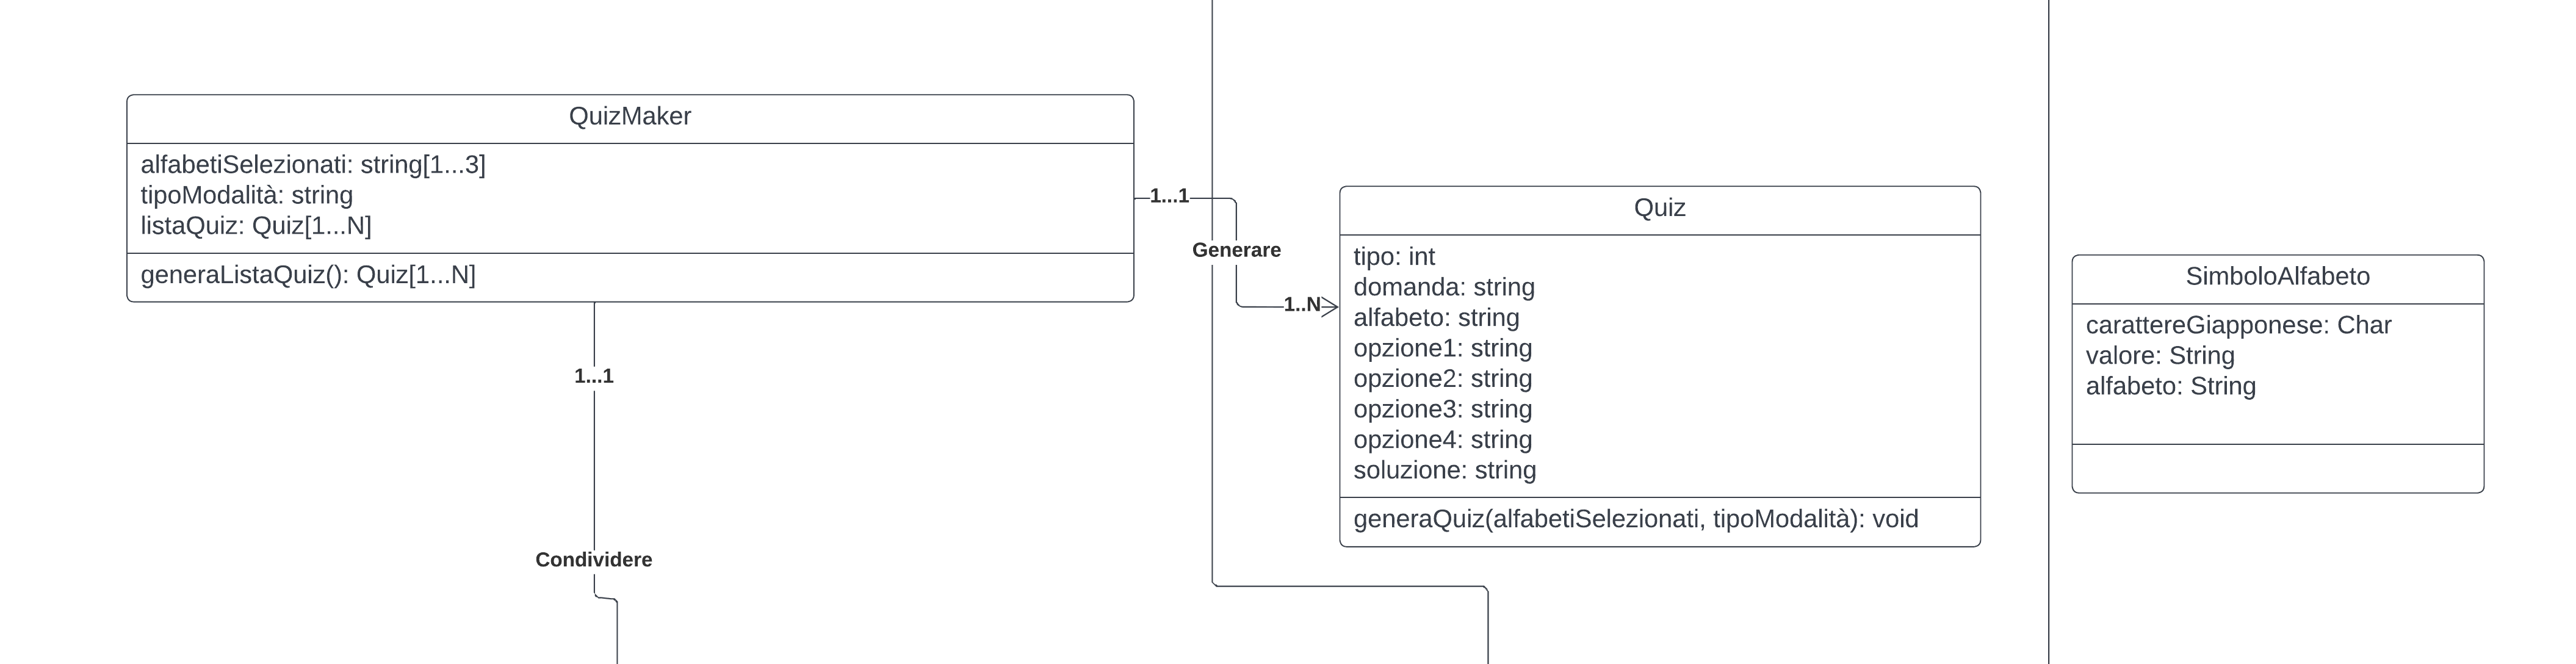
\includegraphics[scale=0.10]{images/classe_quiz_quizmaker.png}
\caption{Gestione creazione quiz}
\label{fig:classe_quizmaker}
\end{figure}
\noindent
La classe QuizMaker si occupa di generare una lista di quiz in base alle informazioni che riceve dal Front-End riguardo le scelte dell'utente, di conseguenza abbiamo la relazione 'generare' tra QuizMaker e Quiz. QuizMaker si occuperà anche di inviare i quiz al Front-End stesso per essere visualizzati e per essere a loro volta inoltrati verso la classe CorrettoreQuiz.

\subsection{Correttore Quiz e Interprete Disegni}
Analizzando il diagramma delle componenti si possono evincere le componenti:
\begin{itemize}
    \item Sistema interpretazione disegno: si occupa di inviare il disegno dell'utente fatto nel quiz di tipo 4, al sistema esterno Nyckel per essere interpretato, riceve indietro una stringa che inoltra nuovamente a paginaQuiz. Questa componente è stata tradotta nella classe InterpreteDisegno, che si interfaccia all'API di Nyckel.
    \item Pagina quiz: riceve dalla componente quizMaker i vari quiz, li fa visualizzare in sequenza all'utente, stabilisce se le risposte di quest'ultimo sono corrette e, nel caso di una sfida online, ordina al Gestore sessione online di far terminare la sfida. la parte di questa componente che si occupa solamente di riceve il quiz, e di verificare la risposta dell'utente è stata tradotta nel diagramma delle classi nella classe CorrettoreQuiz.\\
\end{itemize}
\noindent

\begin{figure}[!h]
\centering
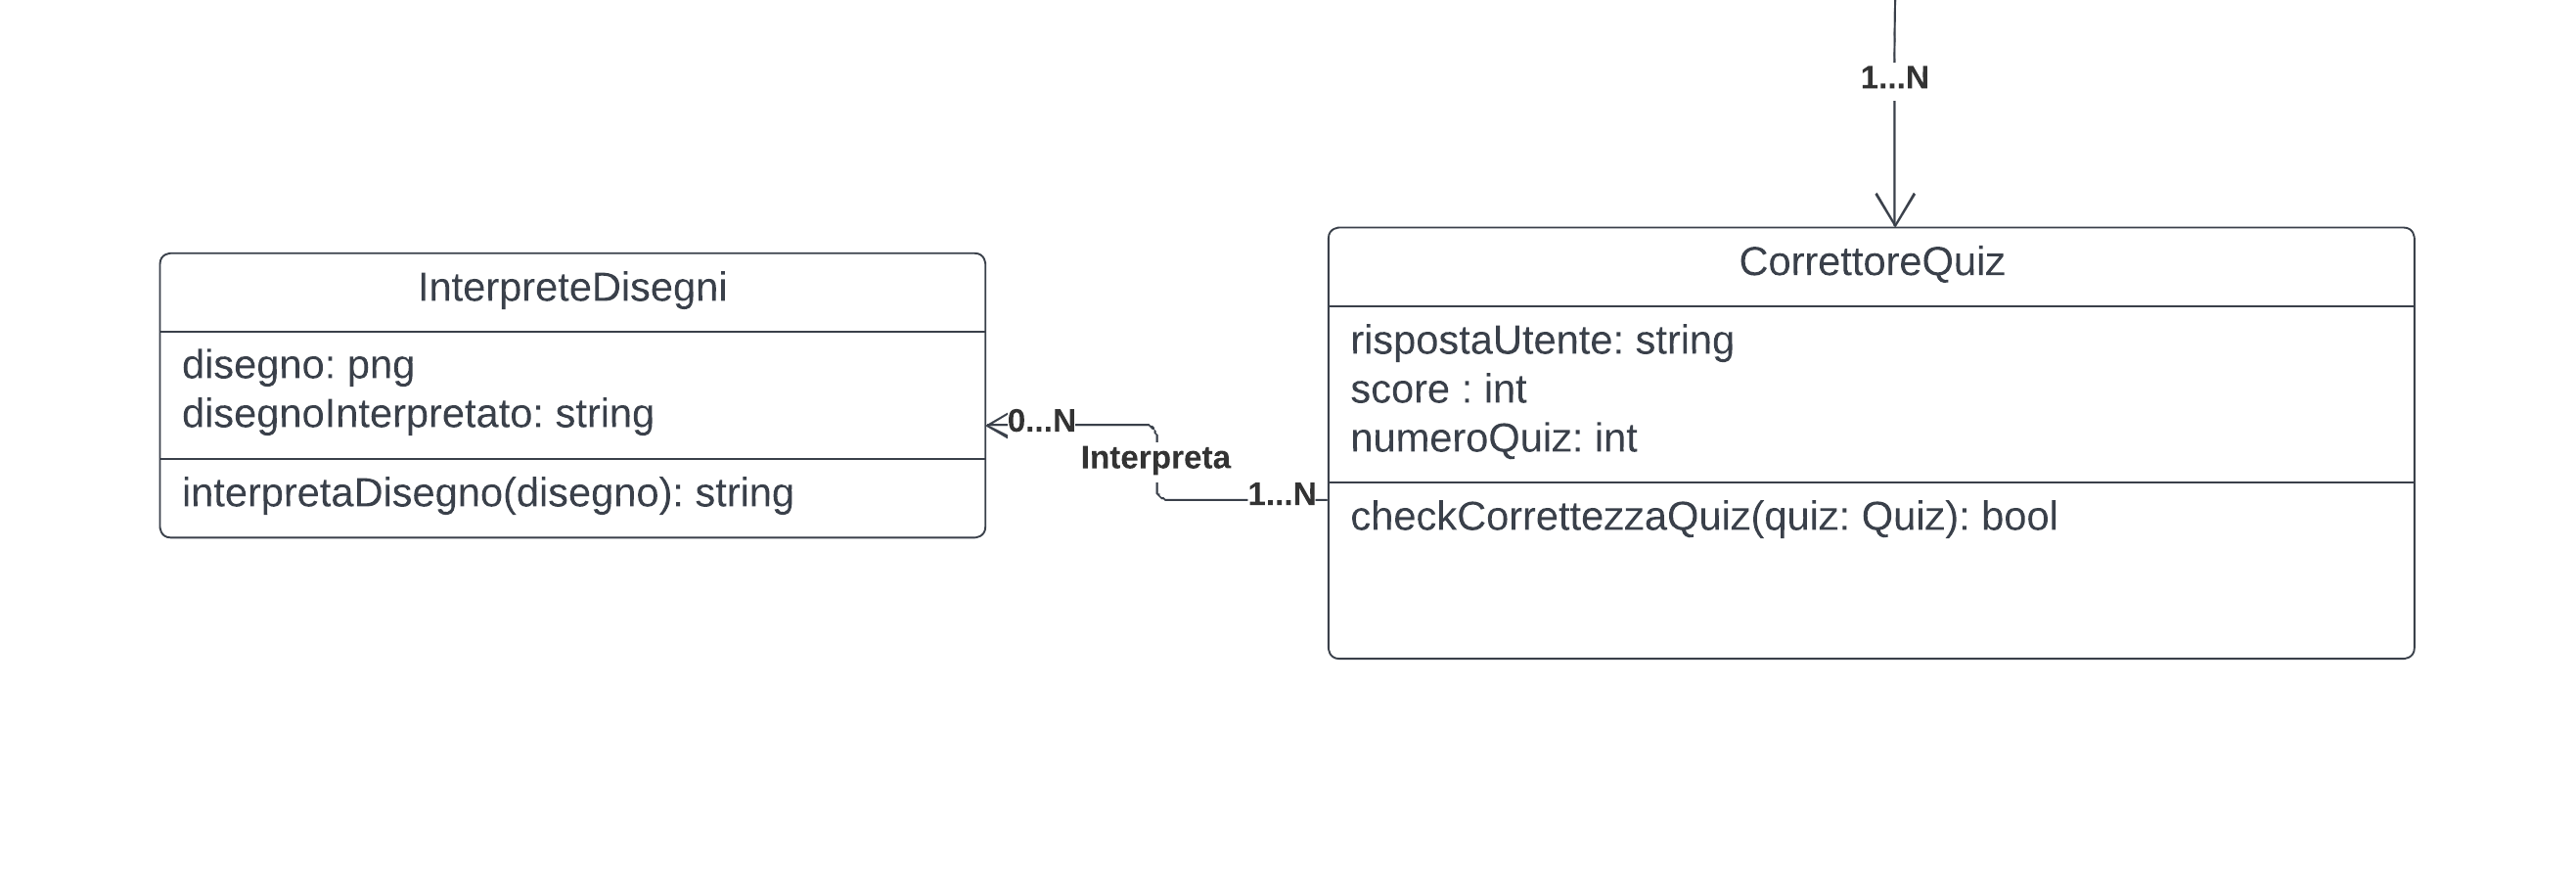
\includegraphics[scale=0.10]{images/classe_correttore_quiz_interprete_disegni.png}
\caption{Correttore quiz}
\label{fig:classe_correttore_quiz}
\end{figure}
\noindent
Inoltre è stata identificata una relazione tra le due classi. Questo perchè nel caso il Correttore quiz debba correggere la risposta ad un quiz di tipo 4 avrà bisogno di interpretare il disegno fornito dall'utente tramite l'Interprete disegno.

\subsection{Sfida Giornaliera}
Si è ritenuto oppurtuno scomporre la componente Pagina quiz del diagramma delle componenti in più classi, una di queste è la classe SfidaGiornaliera.

\begin{figure}[!h]
\centering
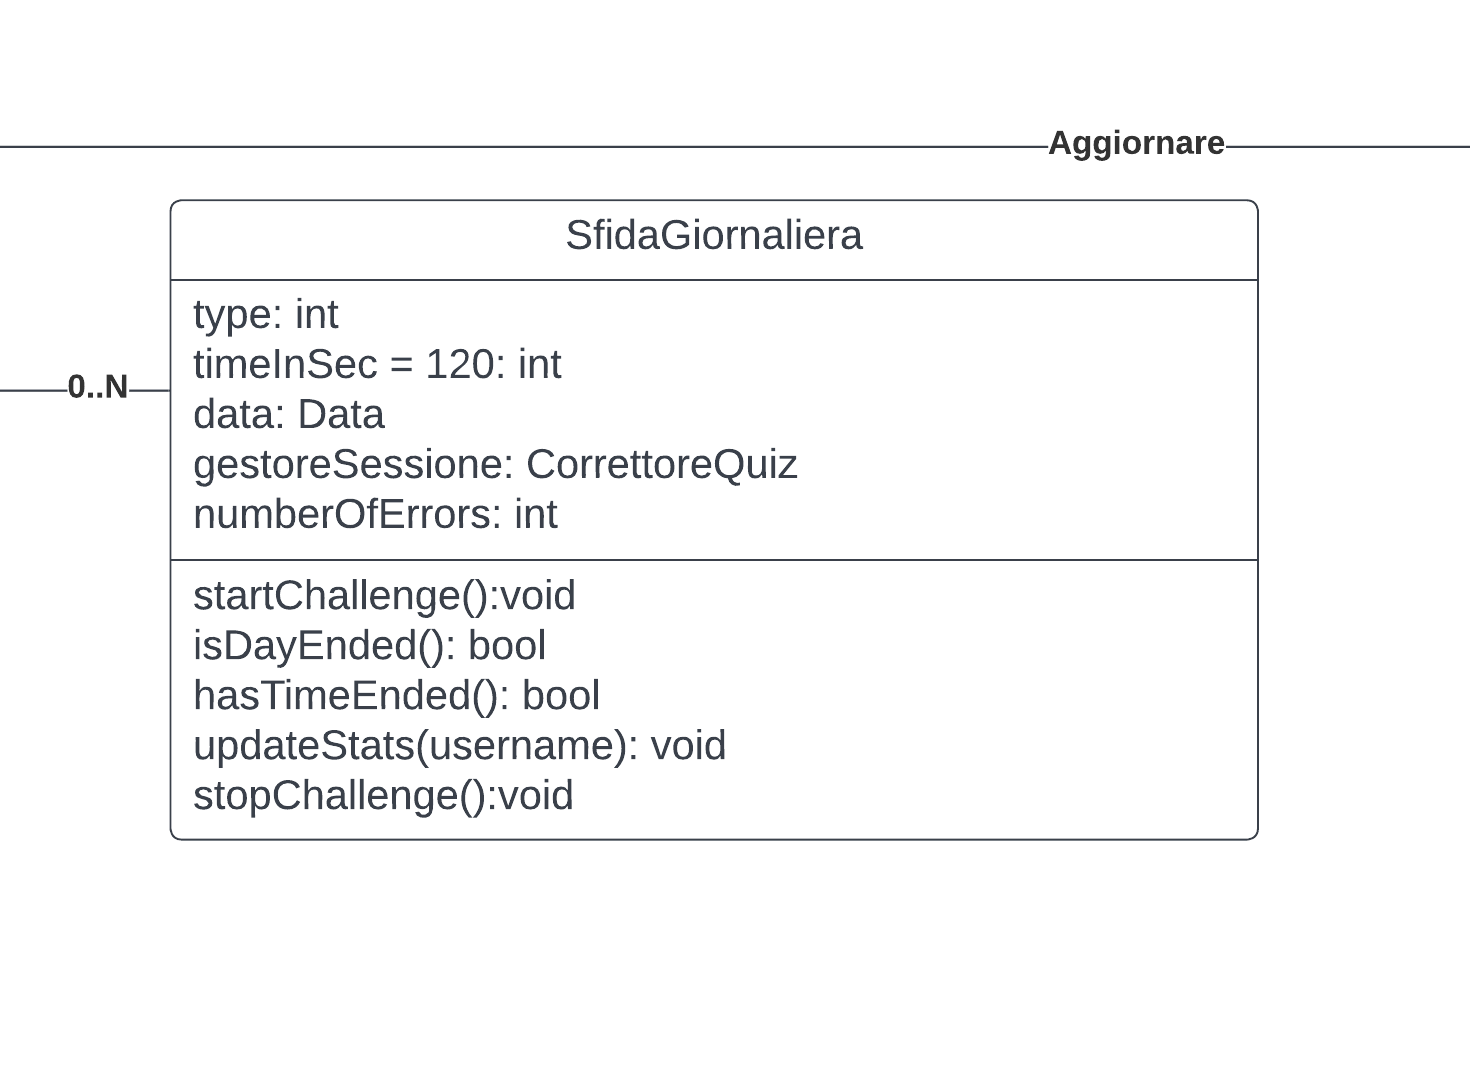
\includegraphics[scale=0.10]{images/classe_sfida_giornaliera.png}
\caption{Classe sfida giornaliera}
\label{fig:classe_sfida_giornaliera}
\end{figure}
\noindent
Questa componente si occupa di correggere le risposte ai quiz della sfida giornaliera di un singolo utente, e di aggiornare le sue statistiche una volta finita la sfida. Per questa ragione la classe istanzia un oggetto di tipo CorrettoreQuiz. L'operazione isDayEnded si occupa di verificare che non sia stata superata la data collegata alla sfida giornaliera che sta visualizzando, in tal caso segna la sfida come persa a priori e aggiorna le statistiche degli utenti di conseguenza. 

\subsection{Sistema di ricerca giocatori, gestione giocatori e inviti}
Analizzando il diagramma delle componenti si possono trovare le seguenti componenti:
\begin{itemize}
    \item Sistema di ricerca giocatori: si occupa di distinguere il tipo di sfida online l'utente vuole fare (casuale o sfidando un giocatore specifico). Se viene inserito uno username verifica la sua validità interfacciandosi con il Database. Nel diagramma delle classi è stato tradotto nella classe omonima. Quest'ultima si occupa anche di istanziare il GestoreGiocatoriDisponibi o il GestoreInivitiSfida a seconda del tipo di ricerca viene effettuata.
    \item Gestore invio inviti di sfida: si occupa di inviare una richiesta di invio invito, questa componente è stata trasformata nella classe GestoreInvitiSfida.
    \item Notifica di sfida: si occupa di inviare l'invito alla sfida all'utente e di inoltrare la risposta di quest'ultimo alla componente pagina multiplayer, questa componente è stata inglobata dalla classe GestoreInvitiSfida che nel suo complesso si occupa di inviare una richiesta di invito al Front-End e di ricevere la risposta dell'utente, nel caso essa sia positiva inoltra verso la classe GestioneSessioneMultiplayer gli username dei due utenti.
    \item Gestore giocatori disponibii: si occupa di aggiornare lo stato dell'utente, e di scegliere un utente casuale tra quelli disponibili per iniziare la sessione di sfida, nel diagramma delle classi diventa la classe GestoreGiocatoriDisponibili che si interfaccia all'API di mongoDB. \\
\end{itemize}

\begin{figure}[!h]
\centering
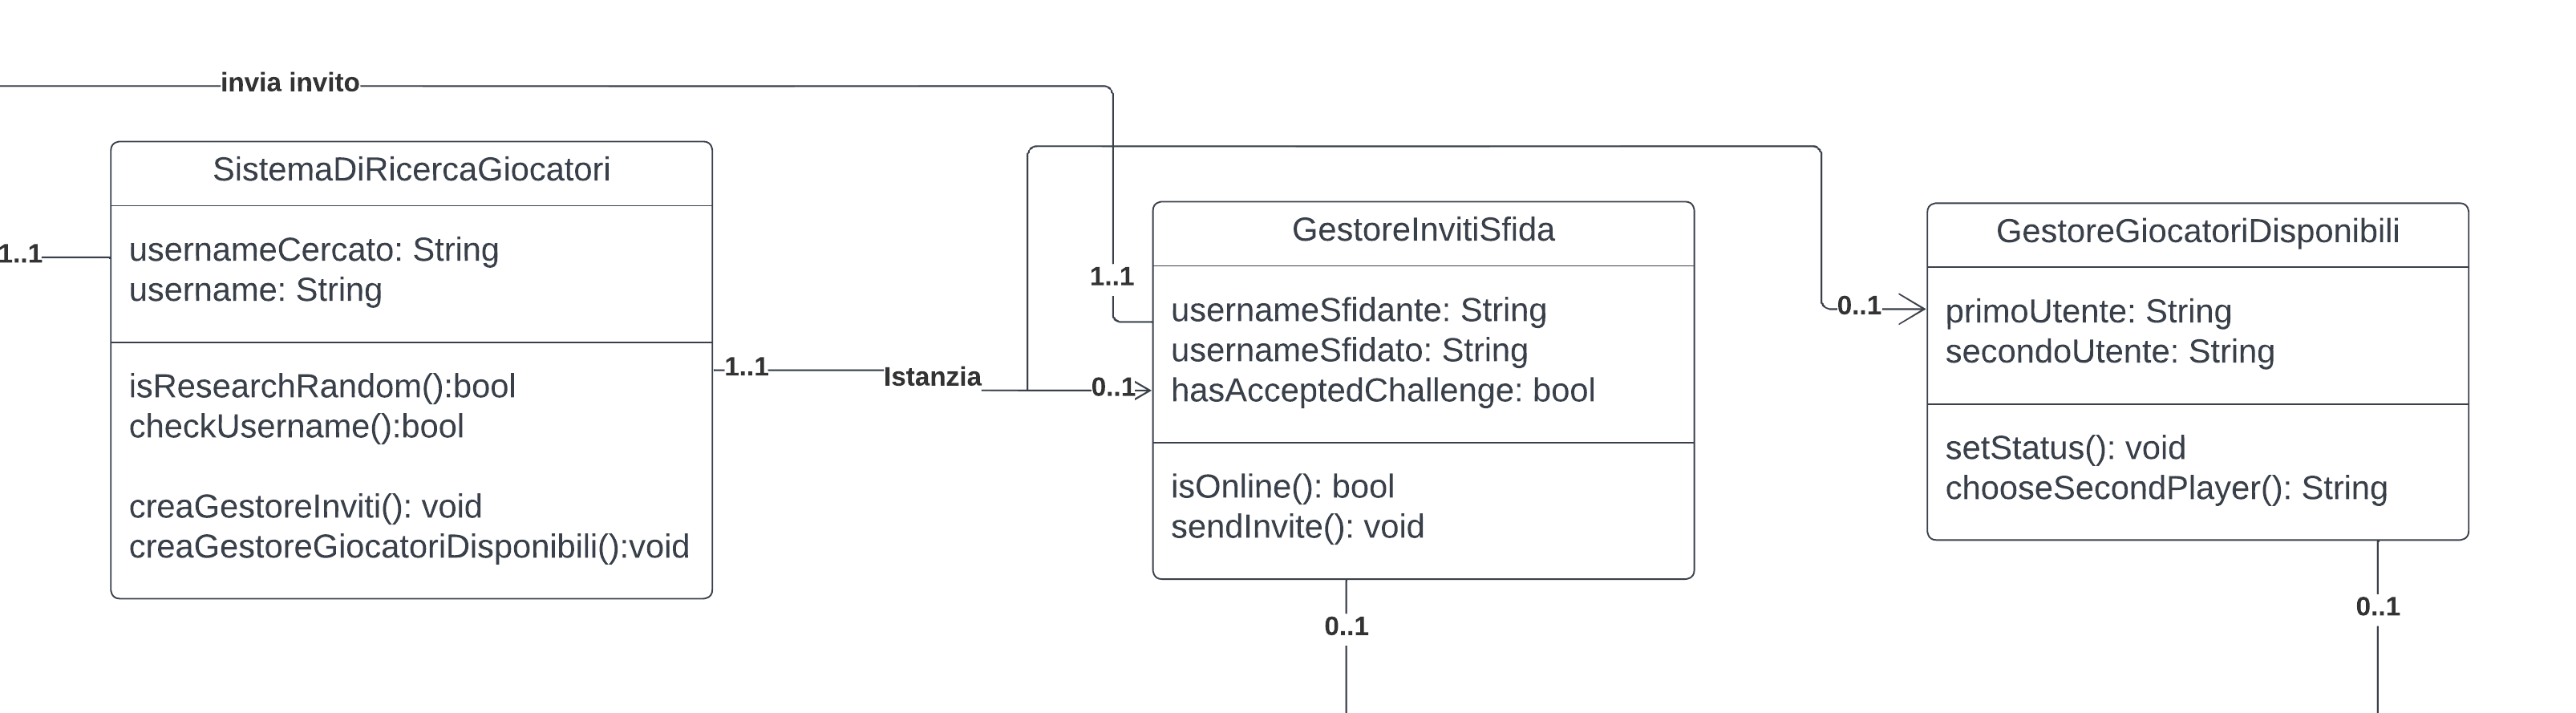
\includegraphics[scale=0.10]{images/classe_ricerca_invita_disponibilita_giocatori.png}
\caption{Gestore ricerca, inviti e disponibilità}
\label{fig:classe_ricerca_inviti_disponibilità}
\end{figure}
\noindent
Sono state individuate anche delle relazioni tra le tre classi, infatti il Sistema di ricerca giocatori è in relazione sia con GestoreGiocatoriDisponibili che con GestoreInvitiSfida attraverso la relazione 'istanziare'.

\subsection{Gestore sessione Multiplayer}
Nel diagramma delle componenti si trovano la classe pagina Multiplayer, quest'ultima si occupa di far visualizzare ai due utenti i quiz, riceve le loro risposte e stabilire i vincitori. Questa componente è stata tradotta nella classe GestoreSessioneMultiplayer per quanto riguarda il suo ruolo nel Back-End, ossia correggere i quiz, e tramite l'API di mongoDB aggioranre il punteggio dei due giocatori e le loro statistiche in base all'esito della sfida. QUesta classe istanzia due oggetti di tipo CorrettoreQuiz, uno per utente. L'operazione stopSession si occupa di far terminare la sfida online una volta che uno dei due giocatori avrà risposto a tutti i quiz della sfida. 

\begin{figure}[!h]
\centering
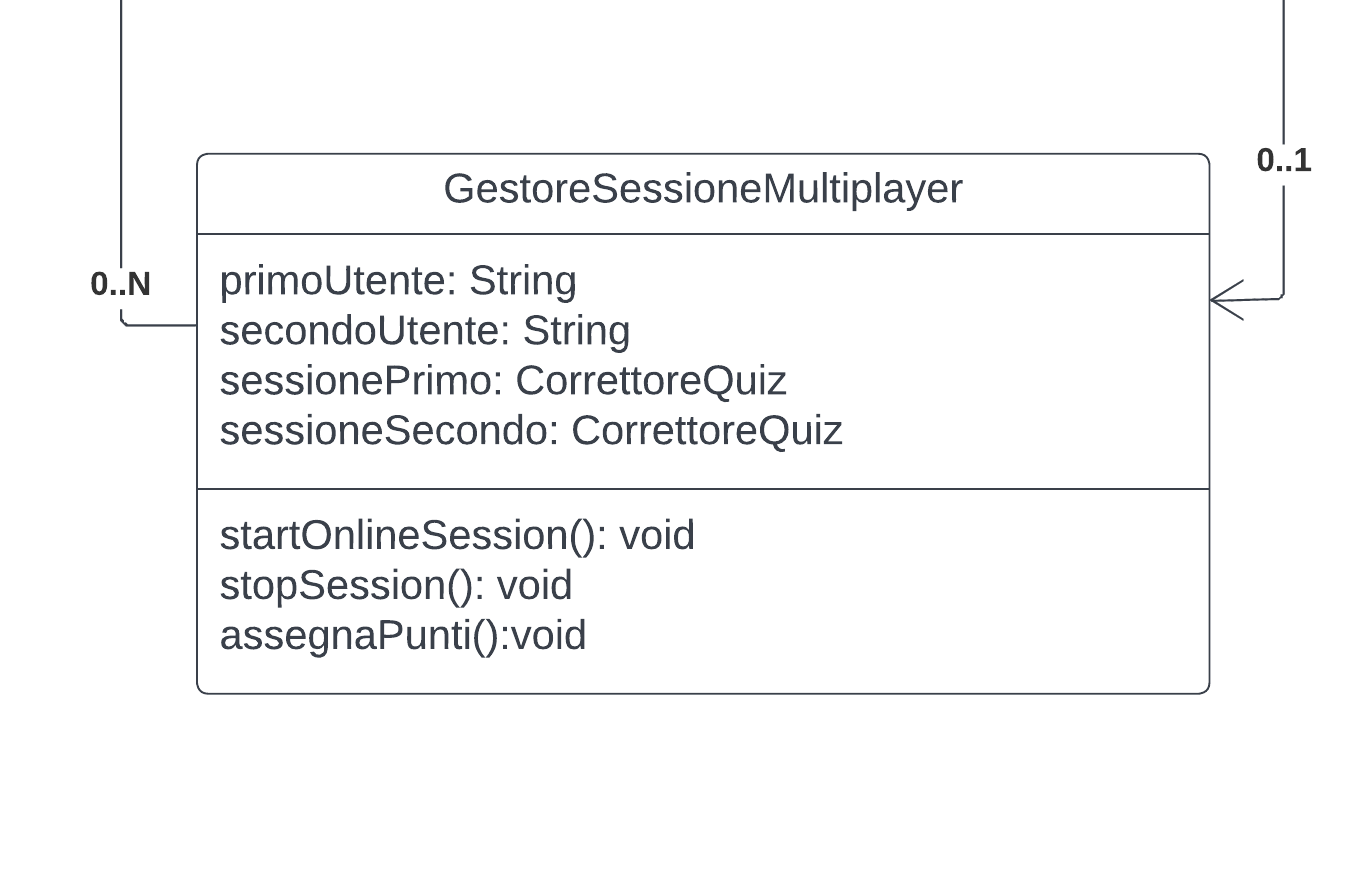
\includegraphics[scale=0.10]{images/classe_gestore_sessione_multiplayer.png}
\caption{Classe gestione multiplayer}
\label{fig:classe_multiplayer}
\end{figure}
\noindent

\newpage
\subsection{Diagramma delle classi complessivo}
\begin{figure}[!h]
\centering
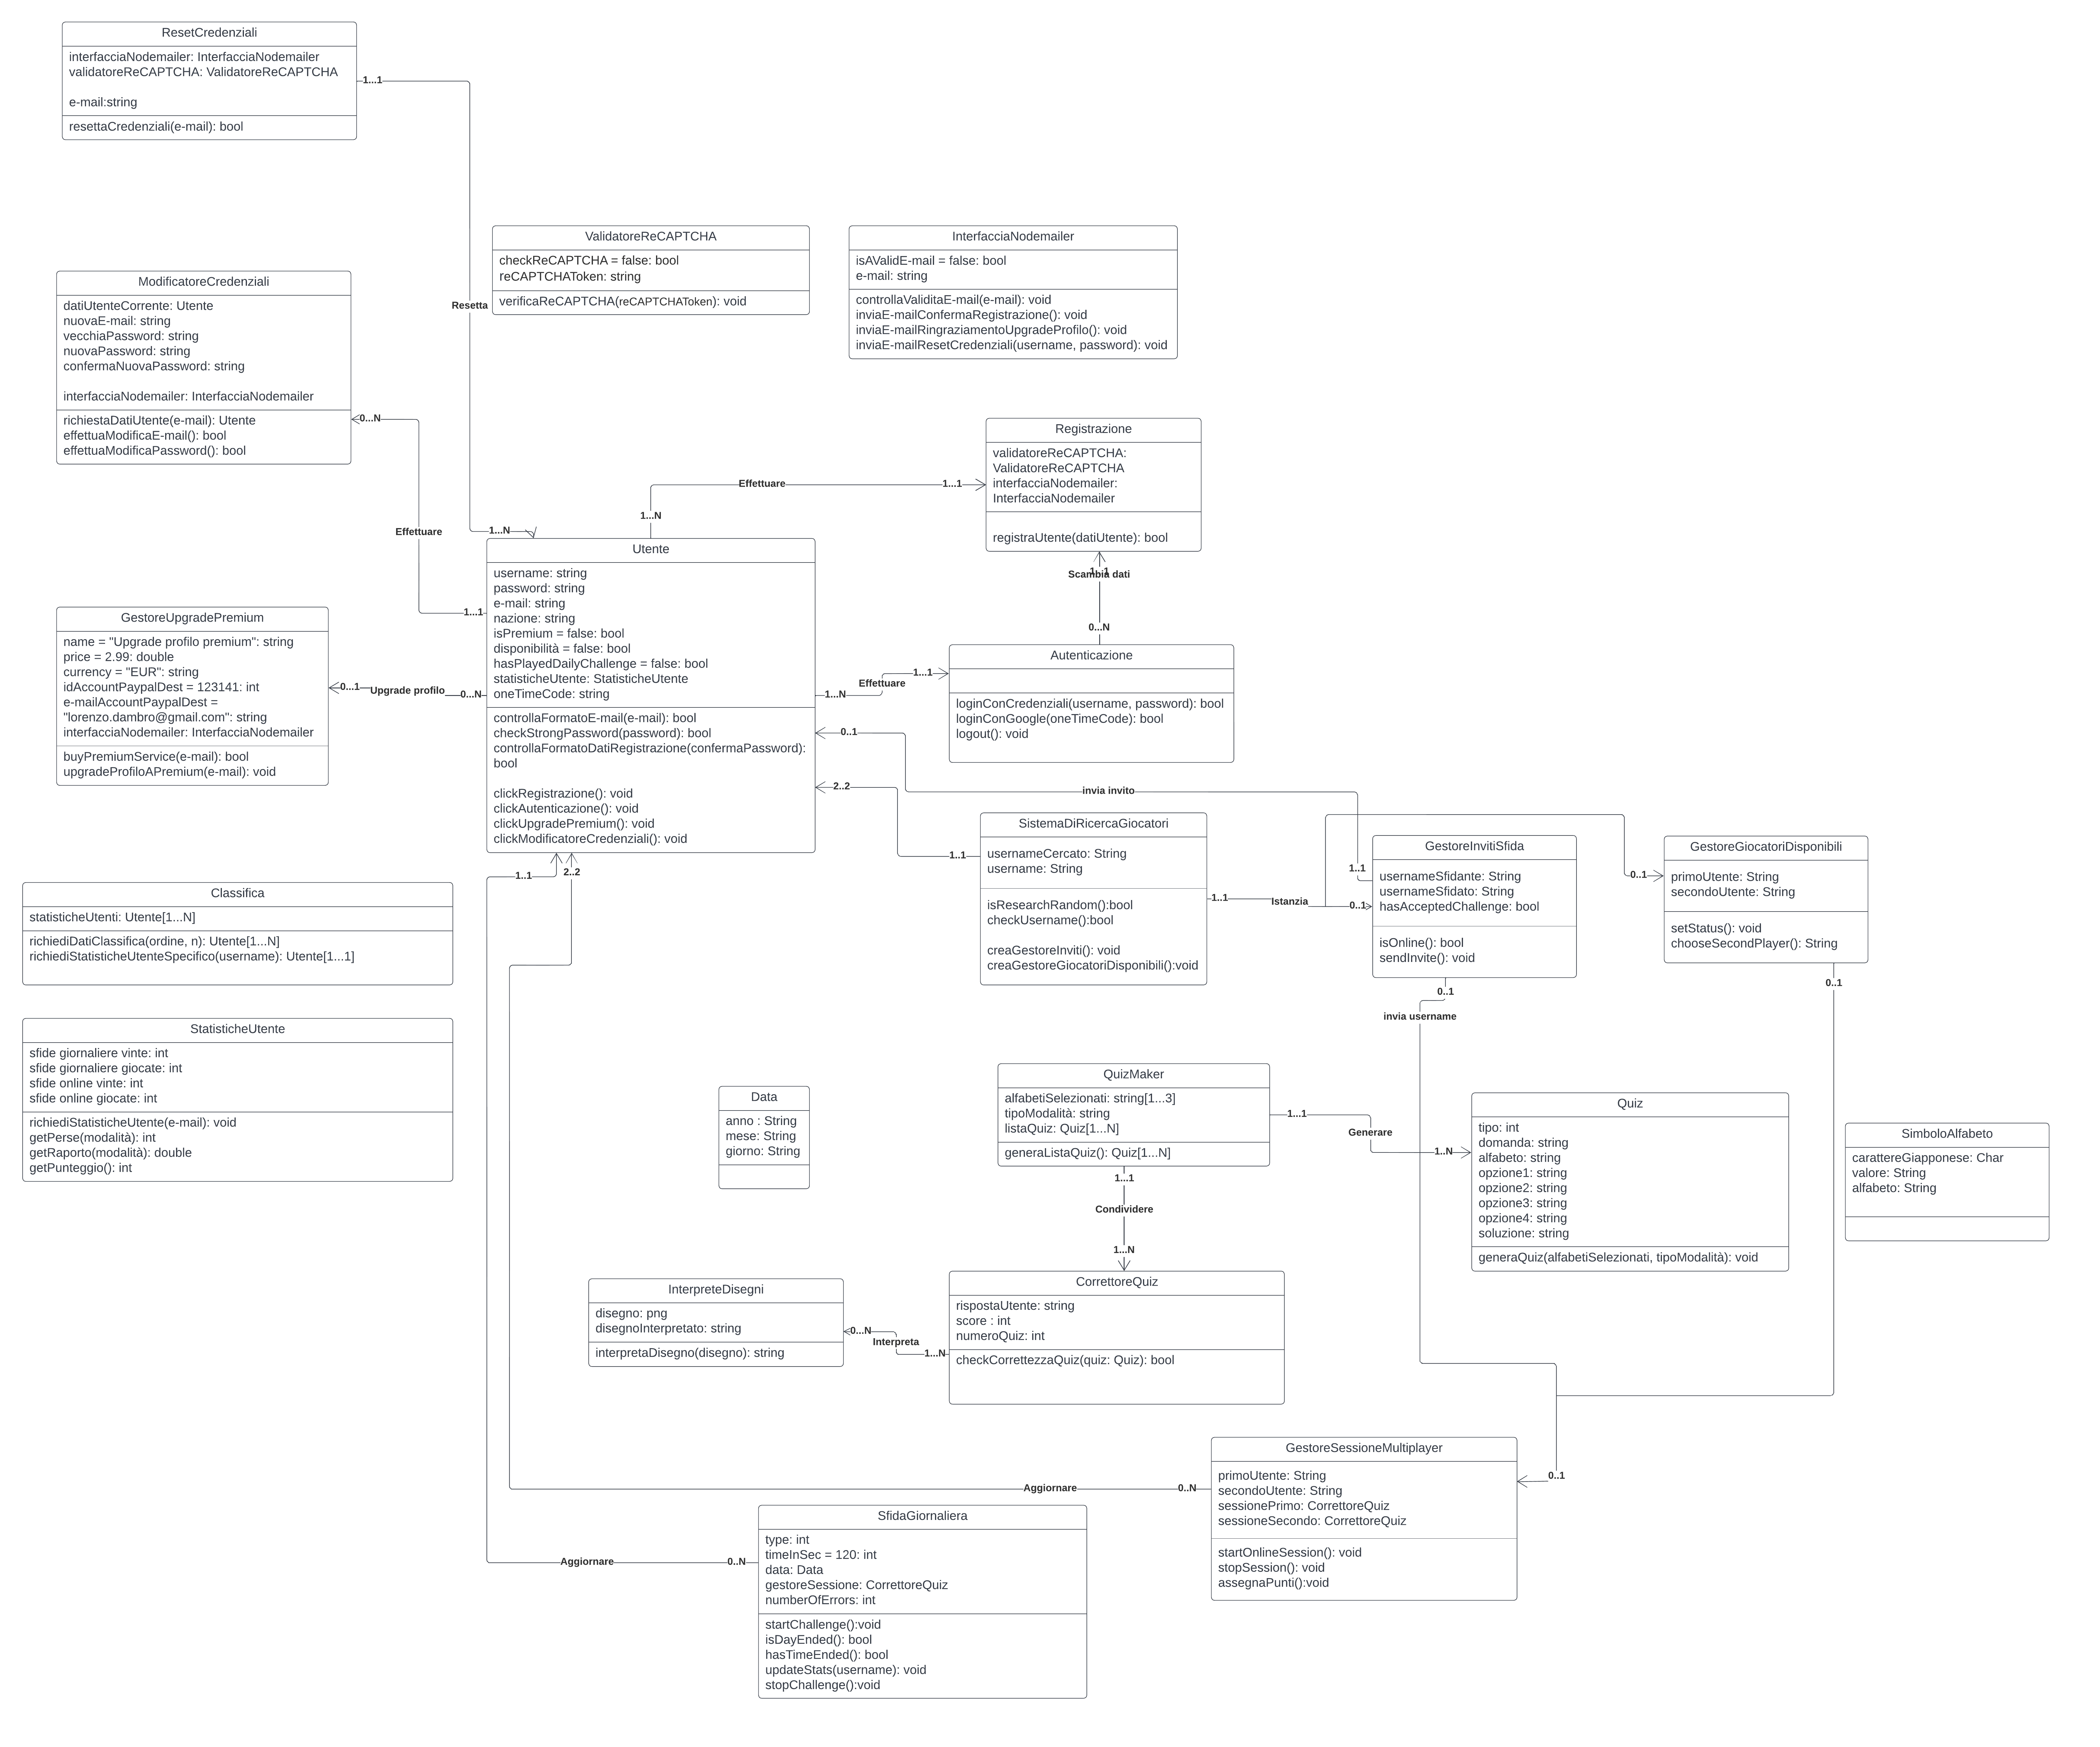
\includegraphics[scale=0.07]{images/diagramma_delle_classi_complessivo.png}
\caption{Diagramma classi completo}
\label{fig:diagramma_classi}
\end{figure}
\noindent